% Created by tikzDevice version 0.12.3.1 on 2023-04-24 13:44:39
% !TEX encoding = UTF-8 Unicode
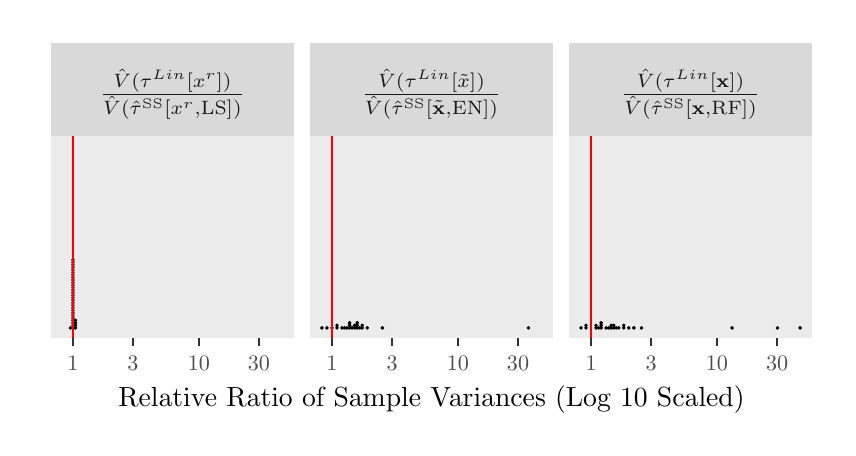
\begin{tikzpicture}[x=1pt,y=1pt]
\definecolor{fillColor}{RGB}{255,255,255}
\path[use as bounding box,fill=fillColor,fill opacity=0.00] (0,0) rectangle (289.08,144.54);
\begin{scope}
\path[clip] (  0.00,  0.00) rectangle (289.08,144.54);
\definecolor{drawColor}{RGB}{255,255,255}
\definecolor{fillColor}{RGB}{255,255,255}

\path[draw=drawColor,line width= 0.6pt,line join=round,line cap=round,fill=fillColor] (  0.00,  0.00) rectangle (289.08,144.54);
\end{scope}
\begin{scope}
\path[clip] (  8.25, 32.28) rectangle ( 96.36,105.24);
\definecolor{fillColor}{gray}{0.92}

\path[fill=fillColor] (  8.25, 32.28) rectangle ( 96.36,105.24);
\definecolor{drawColor}{RGB}{0,0,0}
\definecolor{fillColor}{RGB}{0,0,0}

\path[draw=drawColor,line width= 0.4pt,line join=round,fill=fillColor] ( 15.44, 36.05) circle (  0.46);

\path[draw=drawColor,line width= 0.4pt,line join=round,fill=fillColor] ( 16.35, 36.05) circle (  0.46);

\path[draw=drawColor,line width= 0.4pt,line join=round,fill=fillColor] ( 16.35, 36.96) circle (  0.46);

\path[draw=drawColor,line width= 0.4pt,line join=round,fill=fillColor] ( 16.35, 37.87) circle (  0.46);

\path[draw=drawColor,line width= 0.4pt,line join=round,fill=fillColor] ( 16.35, 38.78) circle (  0.46);

\path[draw=drawColor,line width= 0.4pt,line join=round,fill=fillColor] ( 16.35, 39.69) circle (  0.46);

\path[draw=drawColor,line width= 0.4pt,line join=round,fill=fillColor] ( 16.35, 40.60) circle (  0.46);

\path[draw=drawColor,line width= 0.4pt,line join=round,fill=fillColor] ( 16.35, 41.51) circle (  0.46);

\path[draw=drawColor,line width= 0.4pt,line join=round,fill=fillColor] ( 16.35, 42.42) circle (  0.46);

\path[draw=drawColor,line width= 0.4pt,line join=round,fill=fillColor] ( 16.35, 43.33) circle (  0.46);

\path[draw=drawColor,line width= 0.4pt,line join=round,fill=fillColor] ( 16.35, 44.24) circle (  0.46);

\path[draw=drawColor,line width= 0.4pt,line join=round,fill=fillColor] ( 16.35, 45.15) circle (  0.46);

\path[draw=drawColor,line width= 0.4pt,line join=round,fill=fillColor] ( 16.35, 46.06) circle (  0.46);

\path[draw=drawColor,line width= 0.4pt,line join=round,fill=fillColor] ( 16.35, 46.97) circle (  0.46);

\path[draw=drawColor,line width= 0.4pt,line join=round,fill=fillColor] ( 16.35, 47.88) circle (  0.46);

\path[draw=drawColor,line width= 0.4pt,line join=round,fill=fillColor] ( 16.35, 48.79) circle (  0.46);

\path[draw=drawColor,line width= 0.4pt,line join=round,fill=fillColor] ( 16.35, 49.70) circle (  0.46);

\path[draw=drawColor,line width= 0.4pt,line join=round,fill=fillColor] ( 16.35, 50.61) circle (  0.46);

\path[draw=drawColor,line width= 0.4pt,line join=round,fill=fillColor] ( 16.35, 51.52) circle (  0.46);

\path[draw=drawColor,line width= 0.4pt,line join=round,fill=fillColor] ( 16.35, 52.43) circle (  0.46);

\path[draw=drawColor,line width= 0.4pt,line join=round,fill=fillColor] ( 16.35, 53.34) circle (  0.46);

\path[draw=drawColor,line width= 0.4pt,line join=round,fill=fillColor] ( 16.35, 54.25) circle (  0.46);

\path[draw=drawColor,line width= 0.4pt,line join=round,fill=fillColor] ( 16.35, 55.16) circle (  0.46);

\path[draw=drawColor,line width= 0.4pt,line join=round,fill=fillColor] ( 16.35, 56.07) circle (  0.46);

\path[draw=drawColor,line width= 0.4pt,line join=round,fill=fillColor] ( 16.35, 56.98) circle (  0.46);

\path[draw=drawColor,line width= 0.4pt,line join=round,fill=fillColor] ( 16.35, 57.89) circle (  0.46);

\path[draw=drawColor,line width= 0.4pt,line join=round,fill=fillColor] ( 16.35, 58.80) circle (  0.46);

\path[draw=drawColor,line width= 0.4pt,line join=round,fill=fillColor] ( 16.35, 59.71) circle (  0.46);

\path[draw=drawColor,line width= 0.4pt,line join=round,fill=fillColor] ( 16.35, 60.62) circle (  0.46);

\path[draw=drawColor,line width= 0.4pt,line join=round,fill=fillColor] ( 17.26, 36.05) circle (  0.46);

\path[draw=drawColor,line width= 0.4pt,line join=round,fill=fillColor] ( 17.26, 36.96) circle (  0.46);

\path[draw=drawColor,line width= 0.4pt,line join=round,fill=fillColor] ( 17.26, 37.87) circle (  0.46);

\path[draw=drawColor,line width= 0.4pt,line join=round,fill=fillColor] ( 17.26, 38.78) circle (  0.46);
\definecolor{drawColor}{RGB}{255,0,0}

\path[draw=drawColor,line width= 0.6pt,line join=round] ( 16.35, 32.28) -- ( 16.35,105.24);
\end{scope}
\begin{scope}
\path[clip] (101.86, 32.28) rectangle (189.97,105.24);
\definecolor{fillColor}{gray}{0.92}

\path[fill=fillColor] (101.86, 32.28) rectangle (189.97,105.24);
\definecolor{drawColor}{RGB}{0,0,0}
\definecolor{fillColor}{RGB}{0,0,0}

\path[draw=drawColor,line width= 0.4pt,line join=round,fill=fillColor] (106.32, 36.05) circle (  0.46);

\path[draw=drawColor,line width= 0.4pt,line join=round,fill=fillColor] (108.14, 36.05) circle (  0.46);

\path[draw=drawColor,line width= 0.4pt,line join=round,fill=fillColor] (109.96, 36.05) circle (  0.46);

\path[draw=drawColor,line width= 0.4pt,line join=round,fill=fillColor] (111.78, 36.05) circle (  0.46);

\path[draw=drawColor,line width= 0.4pt,line join=round,fill=fillColor] (111.78, 36.96) circle (  0.46);

\path[draw=drawColor,line width= 0.4pt,line join=round,fill=fillColor] (113.60, 36.05) circle (  0.46);

\path[draw=drawColor,line width= 0.4pt,line join=round,fill=fillColor] (114.51, 36.05) circle (  0.46);

\path[draw=drawColor,line width= 0.4pt,line join=round,fill=fillColor] (115.42, 36.05) circle (  0.46);

\path[draw=drawColor,line width= 0.4pt,line join=round,fill=fillColor] (116.33, 36.05) circle (  0.46);

\path[draw=drawColor,line width= 0.4pt,line join=round,fill=fillColor] (116.33, 36.96) circle (  0.46);

\path[draw=drawColor,line width= 0.4pt,line join=round,fill=fillColor] (116.33, 37.87) circle (  0.46);

\path[draw=drawColor,line width= 0.4pt,line join=round,fill=fillColor] (117.24, 36.05) circle (  0.46);

\path[draw=drawColor,line width= 0.4pt,line join=round,fill=fillColor] (118.15, 36.05) circle (  0.46);

\path[draw=drawColor,line width= 0.4pt,line join=round,fill=fillColor] (118.15, 36.96) circle (  0.46);

\path[draw=drawColor,line width= 0.4pt,line join=round,fill=fillColor] (119.06, 36.05) circle (  0.46);

\path[draw=drawColor,line width= 0.4pt,line join=round,fill=fillColor] (119.06, 36.96) circle (  0.46);

\path[draw=drawColor,line width= 0.4pt,line join=round,fill=fillColor] (119.06, 37.87) circle (  0.46);

\path[draw=drawColor,line width= 0.4pt,line join=round,fill=fillColor] (119.97, 36.05) circle (  0.46);

\path[draw=drawColor,line width= 0.4pt,line join=round,fill=fillColor] (120.88, 36.05) circle (  0.46);

\path[draw=drawColor,line width= 0.4pt,line join=round,fill=fillColor] (120.88, 36.96) circle (  0.46);

\path[draw=drawColor,line width= 0.4pt,line join=round,fill=fillColor] (122.70, 36.05) circle (  0.46);

\path[draw=drawColor,line width= 0.4pt,line join=round,fill=fillColor] (128.17, 36.05) circle (  0.46);

\path[draw=drawColor,line width= 0.4pt,line join=round,fill=fillColor] (180.96, 36.05) circle (  0.46);
\definecolor{drawColor}{RGB}{255,0,0}

\path[draw=drawColor,line width= 0.6pt,line join=round] (109.96, 32.28) -- (109.96,105.24);
\end{scope}
\begin{scope}
\path[clip] (195.47, 32.28) rectangle (283.58,105.24);
\definecolor{fillColor}{gray}{0.92}

\path[fill=fillColor] (195.47, 32.28) rectangle (283.58,105.24);
\definecolor{drawColor}{RGB}{0,0,0}
\definecolor{fillColor}{RGB}{0,0,0}

\path[draw=drawColor,line width= 0.4pt,line join=round,fill=fillColor] (199.93, 36.05) circle (  0.46);

\path[draw=drawColor,line width= 0.4pt,line join=round,fill=fillColor] (201.75, 36.05) circle (  0.46);

\path[draw=drawColor,line width= 0.4pt,line join=round,fill=fillColor] (201.75, 36.96) circle (  0.46);

\path[draw=drawColor,line width= 0.4pt,line join=round,fill=fillColor] (205.39, 36.05) circle (  0.46);

\path[draw=drawColor,line width= 0.4pt,line join=round,fill=fillColor] (205.39, 36.96) circle (  0.46);

\path[draw=drawColor,line width= 0.4pt,line join=round,fill=fillColor] (206.30, 36.05) circle (  0.46);

\path[draw=drawColor,line width= 0.4pt,line join=round,fill=fillColor] (207.21, 36.05) circle (  0.46);

\path[draw=drawColor,line width= 0.4pt,line join=round,fill=fillColor] (207.21, 36.96) circle (  0.46);

\path[draw=drawColor,line width= 0.4pt,line join=round,fill=fillColor] (207.21, 37.87) circle (  0.46);

\path[draw=drawColor,line width= 0.4pt,line join=round,fill=fillColor] (209.03, 36.05) circle (  0.46);

\path[draw=drawColor,line width= 0.4pt,line join=round,fill=fillColor] (209.94, 36.05) circle (  0.46);

\path[draw=drawColor,line width= 0.4pt,line join=round,fill=fillColor] (210.85, 36.05) circle (  0.46);

\path[draw=drawColor,line width= 0.4pt,line join=round,fill=fillColor] (210.85, 36.96) circle (  0.46);

\path[draw=drawColor,line width= 0.4pt,line join=round,fill=fillColor] (211.76, 36.05) circle (  0.46);

\path[draw=drawColor,line width= 0.4pt,line join=round,fill=fillColor] (211.76, 36.96) circle (  0.46);

\path[draw=drawColor,line width= 0.4pt,line join=round,fill=fillColor] (212.67, 36.05) circle (  0.46);

\path[draw=drawColor,line width= 0.4pt,line join=round,fill=fillColor] (213.58, 36.05) circle (  0.46);

\path[draw=drawColor,line width= 0.4pt,line join=round,fill=fillColor] (215.40, 36.05) circle (  0.46);

\path[draw=drawColor,line width= 0.4pt,line join=round,fill=fillColor] (215.40, 36.96) circle (  0.46);

\path[draw=drawColor,line width= 0.4pt,line join=round,fill=fillColor] (217.22, 36.05) circle (  0.46);

\path[draw=drawColor,line width= 0.4pt,line join=round,fill=fillColor] (219.04, 36.05) circle (  0.46);

\path[draw=drawColor,line width= 0.4pt,line join=round,fill=fillColor] (221.78, 36.05) circle (  0.46);

\path[draw=drawColor,line width= 0.4pt,line join=round,fill=fillColor] (254.54, 36.05) circle (  0.46);

\path[draw=drawColor,line width= 0.4pt,line join=round,fill=fillColor] (270.93, 36.05) circle (  0.46);

\path[draw=drawColor,line width= 0.4pt,line join=round,fill=fillColor] (279.12, 36.05) circle (  0.46);
\definecolor{drawColor}{RGB}{255,0,0}

\path[draw=drawColor,line width= 0.6pt,line join=round] (203.57, 32.28) -- (203.57,105.24);
\end{scope}
\begin{scope}
\path[clip] (  8.25,105.24) rectangle ( 96.36,139.04);
\definecolor{fillColor}{gray}{0.85}

\path[fill=fillColor] (  8.25,105.24) rectangle ( 96.36,139.04);
\definecolor{drawColor}{gray}{0.10}

\node[text=drawColor,anchor=base,inner sep=0pt, outer sep=0pt, scale=  1.00] at ( 52.31,125.21) {};

\node[text=drawColor,anchor=base,inner sep=0pt, outer sep=0pt, scale=  1.00] at ( 52.31,118.01) {$\frac{\hat{\mathbb{V}}(\tau^{Lin}[x^r])}{\hat{\mathbb{V}}(\hat{\tau}^{\mathrm{SS}}[x^r,\mathrm{LS}])}$};

\node[text=drawColor,anchor=base,inner sep=0pt, outer sep=0pt, scale=  1.00] at ( 52.31,110.81) {};
\end{scope}
\begin{scope}
\path[clip] (101.86,105.24) rectangle (189.97,139.04);
\definecolor{fillColor}{gray}{0.85}

\path[fill=fillColor] (101.86,105.24) rectangle (189.97,139.04);
\definecolor{drawColor}{gray}{0.10}

\node[text=drawColor,anchor=base,inner sep=0pt, outer sep=0pt, scale=  1.00] at (145.92,125.21) {};

\node[text=drawColor,anchor=base,inner sep=0pt, outer sep=0pt, scale=  1.00] at (145.92,118.01) {$\frac{\hat{\mathbb{V}}(\tau^{Lin}[\tilde{x}])}{\hat{\mathbb{V}}(\hat{\tau}^{\mathrm{SS}}[\tilde{\mathbf{x}},\mathrm{EN}])}$};

\node[text=drawColor,anchor=base,inner sep=0pt, outer sep=0pt, scale=  1.00] at (145.92,110.81) {};
\end{scope}
\begin{scope}
\path[clip] (195.47,105.24) rectangle (283.58,139.04);
\definecolor{fillColor}{gray}{0.85}

\path[fill=fillColor] (195.47,105.24) rectangle (283.58,139.04);
\definecolor{drawColor}{gray}{0.10}

\node[text=drawColor,anchor=base,inner sep=0pt, outer sep=0pt, scale=  1.00] at (239.52,125.21) {};

\node[text=drawColor,anchor=base,inner sep=0pt, outer sep=0pt, scale=  1.00] at (239.52,118.01) {$\frac{\hat{\mathbb{V}}(\tau^{Lin}[\mathbf{x}])}{\hat{\mathbb{V}}(\hat{\tau}^{\mathrm{SS}}[\mathbf{x},\mathrm{RF}])}$};

\node[text=drawColor,anchor=base,inner sep=0pt, outer sep=0pt, scale=  1.00] at (239.52,110.81) {};
\end{scope}
\begin{scope}
\path[clip] (  0.00,  0.00) rectangle (289.08,144.54);
\definecolor{drawColor}{gray}{0.20}

\path[draw=drawColor,line width= 0.6pt,line join=round] ( 16.35, 29.53) --
	( 16.35, 32.28);

\path[draw=drawColor,line width= 0.6pt,line join=round] ( 38.07, 29.53) --
	( 38.07, 32.28);

\path[draw=drawColor,line width= 0.6pt,line join=round] ( 61.86, 29.53) --
	( 61.86, 32.28);

\path[draw=drawColor,line width= 0.6pt,line join=round] ( 83.58, 29.53) --
	( 83.58, 32.28);
\end{scope}
\begin{scope}
\path[clip] (  0.00,  0.00) rectangle (289.08,144.54);
\definecolor{drawColor}{gray}{0.30}

\node[text=drawColor,anchor=base,inner sep=0pt, outer sep=0pt, scale=  0.80] at ( 16.35, 20.71) {1};

\node[text=drawColor,anchor=base,inner sep=0pt, outer sep=0pt, scale=  0.80] at ( 38.07, 20.71) {3};

\node[text=drawColor,anchor=base,inner sep=0pt, outer sep=0pt, scale=  0.80] at ( 61.86, 20.71) {10};

\node[text=drawColor,anchor=base,inner sep=0pt, outer sep=0pt, scale=  0.80] at ( 83.58, 20.71) {30};
\end{scope}
\begin{scope}
\path[clip] (  0.00,  0.00) rectangle (289.08,144.54);
\definecolor{drawColor}{gray}{0.20}

\path[draw=drawColor,line width= 0.6pt,line join=round] (109.96, 29.53) --
	(109.96, 32.28);

\path[draw=drawColor,line width= 0.6pt,line join=round] (131.68, 29.53) --
	(131.68, 32.28);

\path[draw=drawColor,line width= 0.6pt,line join=round] (155.47, 29.53) --
	(155.47, 32.28);

\path[draw=drawColor,line width= 0.6pt,line join=round] (177.19, 29.53) --
	(177.19, 32.28);
\end{scope}
\begin{scope}
\path[clip] (  0.00,  0.00) rectangle (289.08,144.54);
\definecolor{drawColor}{gray}{0.30}

\node[text=drawColor,anchor=base,inner sep=0pt, outer sep=0pt, scale=  0.80] at (109.96, 20.71) {1};

\node[text=drawColor,anchor=base,inner sep=0pt, outer sep=0pt, scale=  0.80] at (131.68, 20.71) {3};

\node[text=drawColor,anchor=base,inner sep=0pt, outer sep=0pt, scale=  0.80] at (155.47, 20.71) {10};

\node[text=drawColor,anchor=base,inner sep=0pt, outer sep=0pt, scale=  0.80] at (177.19, 20.71) {30};
\end{scope}
\begin{scope}
\path[clip] (  0.00,  0.00) rectangle (289.08,144.54);
\definecolor{drawColor}{gray}{0.20}

\path[draw=drawColor,line width= 0.6pt,line join=round] (203.57, 29.53) --
	(203.57, 32.28);

\path[draw=drawColor,line width= 0.6pt,line join=round] (225.29, 29.53) --
	(225.29, 32.28);

\path[draw=drawColor,line width= 0.6pt,line join=round] (249.08, 29.53) --
	(249.08, 32.28);

\path[draw=drawColor,line width= 0.6pt,line join=round] (270.80, 29.53) --
	(270.80, 32.28);
\end{scope}
\begin{scope}
\path[clip] (  0.00,  0.00) rectangle (289.08,144.54);
\definecolor{drawColor}{gray}{0.30}

\node[text=drawColor,anchor=base,inner sep=0pt, outer sep=0pt, scale=  0.80] at (203.57, 20.71) {1};

\node[text=drawColor,anchor=base,inner sep=0pt, outer sep=0pt, scale=  0.80] at (225.29, 20.71) {3};

\node[text=drawColor,anchor=base,inner sep=0pt, outer sep=0pt, scale=  0.80] at (249.08, 20.71) {10};

\node[text=drawColor,anchor=base,inner sep=0pt, outer sep=0pt, scale=  0.80] at (270.80, 20.71) {30};
\end{scope}
\begin{scope}
\path[clip] (  0.00,  0.00) rectangle (289.08,144.54);
\definecolor{drawColor}{RGB}{0,0,0}

\node[text=drawColor,anchor=base,inner sep=0pt, outer sep=0pt, scale=  1.00] at (145.91,  7.83) {Relative Ratio of Sample Variances (Log 10 Scaled)};
\end{scope}
\end{tikzpicture}
